\documentclass[10pt]{article}

\usepackage[a3paper,landscape,margin=10mm]{geometry}
\usepackage[T1]{fontenc}
\usepackage{lmodern}
\usepackage{xcolor}
\usepackage{enumitem}
\usepackage{tikz}
\usetikzlibrary{arrows.meta,positioning,calc}

\pagestyle{empty}
\setlength{\parindent}{0pt}

\definecolor{stageblue}{HTML}{DCEBFA}
\definecolor{stagecyan}{HTML}{DDF3F1}
\definecolor{stageviolet}{HTML}{ECE5F6}
\definecolor{stageorange}{HTML}{FBE9D2}
\definecolor{stagerose}{HTML}{F7E2EA}
\definecolor{stagegreen}{HTML}{E0F1E5}
\definecolor{stagegold}{HTML}{F7EECF}
\definecolor{ink}{HTML}{17324D}
\definecolor{muted}{HTML}{516579}

\tikzset{
  topstage/.style={
    rounded corners=3mm,
    draw=ink!75,
    line width=0.9pt,
    text width=8.25cm,
    minimum height=9.85cm,
    inner sep=4mm,
    align=left,
    font=\sffamily\footnotesize,
  },
  bottomstage/.style={
    rounded corners=3mm,
    draw=ink!75,
    line width=0.9pt,
    text width=11.15cm,
    minimum height=9.65cm,
    inner sep=4.5mm,
    align=left,
    font=\sffamily\footnotesize,
  },
  mainarrow/.style={
    -{Stealth[length=3.2mm,width=2.2mm]},
    draw=ink,
    line width=1.15pt,
    rounded corners=2mm,
  },
  feedback/.style={
    -{Stealth[length=3mm,width=2mm]},
    draw=muted,
    line width=0.95pt,
    dashed,
    rounded corners=2mm,
  },
  arrowlabel/.style={
    fill=white,
    inner sep=1.5mm,
    font=\sffamily\scriptsize,
    text=muted,
    align=center,
  }
}

\newcommand{\stageheading}[2]{%
  {\color{ink}\hyphenpenalty=10000\exhyphenpenalty=10000\fontsize{13.5}{15.5}\selectfont\bfseries #1. #2}\par\vspace{1.5mm}%
}
\newcommand{\labeltext}[1]{\textcolor{ink}{\bfseries #1}}

\begin{document}

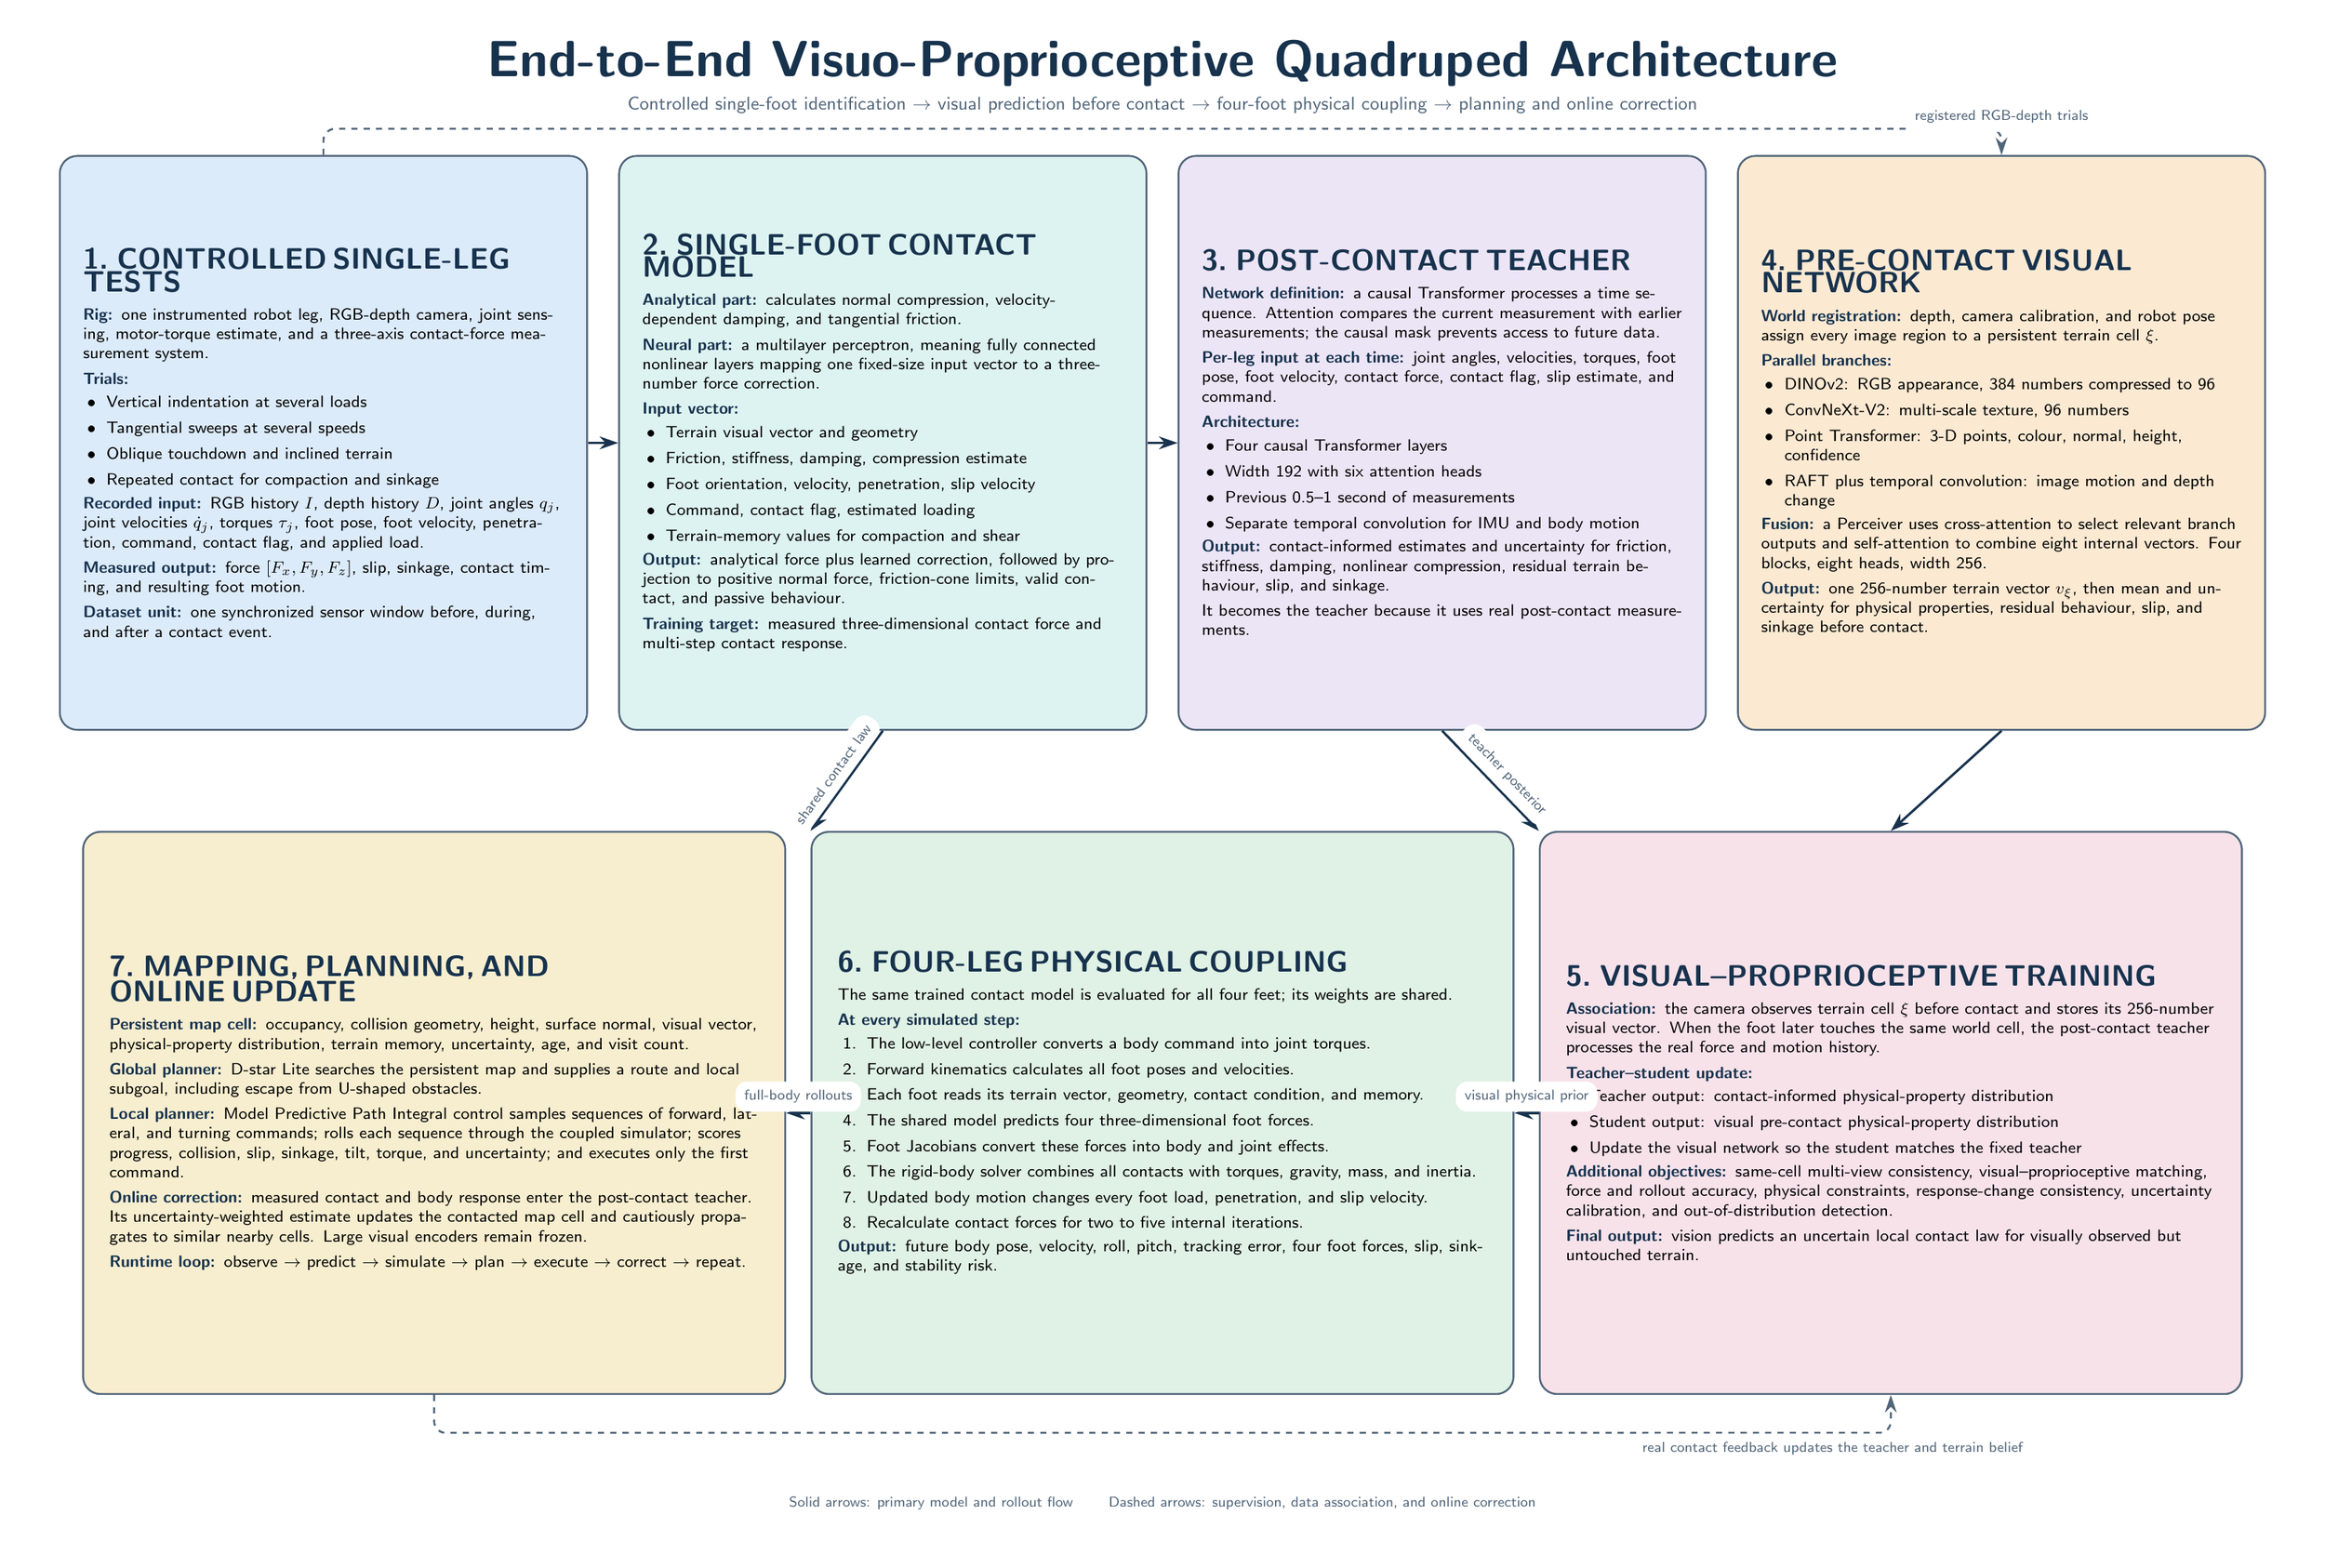
\begin{tikzpicture}[x=1cm,y=1cm]
  \path[use as bounding box] (-19.6,-13.1) rectangle (19.6,13.1);

  \node[font=\sffamily\bfseries\fontsize{24}{28}\selectfont,text=ink]
    at (0,12.35) {End-to-End Visuo-Proprioceptive Quadruped Architecture};
  \node[font=\sffamily\small,text=muted]
    at (0,11.65) {Controlled single-foot identification $\rightarrow$ visual prediction before contact $\rightarrow$ four-foot physical coupling $\rightarrow$ planning and online correction};

  \node[topstage,fill=stageblue] (s1) at (-14.4,5.85) {%
    \stageheading{1}{CONTROLLED \mbox{SINGLE-LEG}\\TESTS}
    \labeltext{Rig:} one instrumented robot leg, RGB-depth camera, joint sensing, motor-torque estimate, and a three-axis contact-force measurement system.\par\vspace{1mm}

    \labeltext{Trials:}
    \begin{itemize}[leftmargin=4mm,itemsep=0.4mm,topsep=0.7mm]
      \item Vertical indentation at several loads
      \item Tangential sweeps at several speeds
      \item Oblique touchdown and inclined terrain
      \item Repeated contact for compaction and sinkage
    \end{itemize}

    \labeltext{Recorded input:} RGB history $I$, depth history $D$, joint angles $q_j$, joint velocities $\dot q_j$, torques $\tau_j$, foot pose, foot velocity, penetration, command, contact flag, and applied load.\par\vspace{1mm}

    \labeltext{Measured output:} force $[F_x,F_y,F_z]$, slip, sinkage, contact timing, and resulting foot motion.\par\vspace{1mm}

    \labeltext{Dataset unit:} one synchronized sensor window before, during, and after a contact event.
  };

  \node[topstage,fill=stagecyan] (s2) at (-4.8,5.85) {%
    \stageheading{2}{\mbox{SINGLE-FOOT} CONTACT\\MODEL}
    \labeltext{Analytical part:} calculates normal compression, velocity-dependent damping, and tangential friction.\par\vspace{1mm}

    \labeltext{Neural part:} a multilayer perceptron, meaning fully connected nonlinear layers mapping one fixed-size input vector to a three-number force correction.\par\vspace{1mm}

    \labeltext{Input vector:}
    \begin{itemize}[leftmargin=4mm,itemsep=0.4mm,topsep=0.7mm]
      \item Terrain visual vector and geometry
      \item Friction, stiffness, damping, compression estimate
      \item Foot orientation, velocity, penetration, slip velocity
      \item Command, contact flag, estimated loading
      \item Terrain-memory values for compaction and shear
    \end{itemize}

    \labeltext{Output:} analytical force plus learned correction, followed by projection to positive normal force, friction-cone limits, valid contact, and passive behaviour.\par\vspace{1mm}

    \labeltext{Training target:} measured three-dimensional contact force and multi-step contact response.
  };

  \node[topstage,fill=stageviolet] (s3) at (4.8,5.85) {%
    \stageheading{3}{\mbox{POST-CONTACT} TEACHER}
    \labeltext{Network definition:} a causal Transformer processes a time sequence. Attention compares the current measurement with earlier measurements; the causal mask prevents access to future data.\par\vspace{1mm}

    \labeltext{Per-leg input at each time:} joint angles, velocities, torques, foot pose, foot velocity, contact force, contact flag, slip estimate, and command.\par\vspace{1mm}

    \labeltext{Architecture:}
    \begin{itemize}[leftmargin=4mm,itemsep=0.4mm,topsep=0.7mm]
      \item Four causal Transformer layers
      \item Width 192 with six attention heads
      \item Previous 0.5--1 second of measurements
      \item Separate temporal convolution for IMU and body motion
    \end{itemize}

    \labeltext{Output:} contact-informed estimates and uncertainty for friction, stiffness, damping, nonlinear compression, residual terrain behaviour, slip, and sinkage.\par\vspace{1mm}

    It becomes the teacher because it uses real post-contact measurements.
  };

  \node[topstage,fill=stageorange] (s4) at (14.4,5.85) {%
    \stageheading{4}{\mbox{PRE-CONTACT} VISUAL\\NETWORK}
    \labeltext{World registration:} depth, camera calibration, and robot pose assign every image region to a persistent terrain cell $\xi$.\par\vspace{1mm}

    \labeltext{Parallel branches:}
    \begin{itemize}[leftmargin=4mm,itemsep=0.4mm,topsep=0.7mm]
      \item DINOv2: RGB appearance, 384 numbers compressed to 96
      \item ConvNeXt-V2: multi-scale texture, 96 numbers
      \item Point Transformer: 3-D points, colour, normal, height, confidence
      \item RAFT plus temporal convolution: image motion and depth change
    \end{itemize}

    \labeltext{Fusion:} a Perceiver uses cross-attention to select relevant branch outputs and self-attention to combine eight internal vectors. Four blocks, eight heads, width 256.\par\vspace{1mm}

    \labeltext{Output:} one 256-number terrain vector $v_\xi$, then mean and uncertainty for physical properties, residual behaviour, slip, and sinkage before contact.
  };

  \node[bottomstage,fill=stagerose] (s5) at (12.5,-5.65) {%
    \stageheading{5}{\mbox{VISUAL--PROPRIOCEPTIVE} TRAINING}
    \labeltext{Association:} the camera observes terrain cell $\xi$ before contact and stores its 256-number visual vector. When the foot later touches the same world cell, the post-contact teacher processes the real force and motion history.\par\vspace{1mm}

    \labeltext{Teacher--student update:}
    \begin{itemize}[leftmargin=4mm,itemsep=0.4mm,topsep=0.7mm]
      \item Teacher output: contact-informed physical-property distribution
      \item Student output: visual pre-contact physical-property distribution
      \item Update the visual network so the student matches the fixed teacher
    \end{itemize}

    \labeltext{Additional objectives:} same-cell multi-view consistency, visual--proprioceptive matching, force and rollout accuracy, physical constraints, response-change consistency, uncertainty calibration, and out-of-distribution detection.\par\vspace{1mm}

    \labeltext{Final output:} vision predicts an uncertain local contact law for visually observed but untouched terrain.
  };

  \node[bottomstage,fill=stagegreen] (s6) at (0,-5.65) {%
    \stageheading{6}{\mbox{FOUR-LEG} PHYSICAL COUPLING}
    The same trained contact model is evaluated for all four feet; its weights are shared.\par\vspace{1mm}

    \labeltext{At every simulated step:}
    \begin{enumerate}[leftmargin=5mm,itemsep=0.35mm,topsep=0.7mm]
      \item The low-level controller converts a body command into joint torques.
      \item Forward kinematics calculates all foot poses and velocities.
      \item Each foot reads its terrain vector, geometry, contact condition, and memory.
      \item The shared model predicts four three-dimensional foot forces.
      \item Foot Jacobians convert these forces into body and joint effects.
      \item The rigid-body solver combines all contacts with torques, gravity, mass, and inertia.
      \item Updated body motion changes every foot load, penetration, and slip velocity.
      \item Recalculate contact forces for two to five internal iterations.
    \end{enumerate}

    \labeltext{Output:} future body pose, velocity, roll, pitch, tracking error, four foot forces, slip, sinkage, and stability risk.
  };

  \node[bottomstage,fill=stagegold] (s7) at (-12.5,-5.65) {%
    \stageheading{7}{MAPPING, PLANNING, AND\\ONLINE UPDATE}
    \labeltext{Persistent map cell:} occupancy, collision geometry, height, surface normal, visual vector, physical-property distribution, terrain memory, uncertainty, age, and visit count.\par\vspace{1mm}

    \labeltext{Global planner:} D-star Lite searches the persistent map and supplies a route and local subgoal, including escape from U-shaped obstacles.\par\vspace{1mm}

    \labeltext{Local planner:} Model Predictive Path Integral control samples sequences of forward, lateral, and turning commands; rolls each sequence through the coupled simulator; scores progress, collision, slip, sinkage, tilt, torque, and uncertainty; and executes only the first command.\par\vspace{1mm}

    \labeltext{Online correction:} measured contact and body response enter the post-contact teacher. Its uncertainty-weighted estimate updates the contacted map cell and cautiously propagates to similar nearby cells. Large visual encoders remain frozen.\par\vspace{1mm}

    \labeltext{Runtime loop:} observe $\rightarrow$ predict $\rightarrow$ simulate $\rightarrow$ plan $\rightarrow$ execute $\rightarrow$ correct $\rightarrow$ repeat.
  };

  % Primary data and model flow
  \draw[mainarrow] (s1.east) -- (s2.west);
  \draw[mainarrow] (s2.east) -- (s3.west);
  \draw[mainarrow] (s4.south) -- (s5.north);
  \draw[mainarrow] (s5.west) -- node[arrowlabel,above]{visual physical prior} (s6.east);
  \draw[mainarrow] (s6.west) -- node[arrowlabel,above]{full-body rollouts} (s7.east);

  % Cross-stream supervision and model transfer
  \draw[feedback] (s1.north) -- ++(0,0.45) -| node[arrowlabel,pos=0.58,above]{registered RGB-depth trials} (s4.north);
  \draw[mainarrow] (s3.south) -- node[arrowlabel,pos=0.55,sloped,above]{teacher posterior} (s5.north west);
  \draw[mainarrow] (s2.south) -- node[arrowlabel,pos=0.52,sloped,above]{shared contact law} (s6.north west);

  % Online contact feedback loop
  \draw[feedback] (s7.south) -- ++(0,-0.65) -| node[arrowlabel,pos=0.48,below]{real contact feedback updates the teacher and terrain belief} (s5.south);

  \node[font=\sffamily\scriptsize,text=muted,align=center] at (0,-12.35)
    {Solid arrows: primary model and rollout flow \qquad Dashed arrows: supervision, data association, and online correction};

\end{tikzpicture}

\end{document}
